\section{Data Sources and Methods}
\label{sec:data_sources_methods}

\subsection{Hydrological Data: AIS GMVO}
\subsubsection{Data Source and Selection Criteria}
Daily discharge and water level observations were obtained from the Automated Information System of State Monitoring of Water Bodies (AIS GMVO), operated by Roshydromet~\citep{AIS_GMVO}.
The database provides stage-discharge records for approximately 3000 active gauging stations across Russia.
The final dataset includes \ndischarge discharge gauging stations and \nwaterlevel water level gauges across \ntotal delineated watersheds.
Selection criteria:
\begin{itemize}
    \item Minimum 10 years of available records between \years
    \item Data completeness $>$80\% during the study period for high-quality subset (\nhighquality gauges)
    \item Quality flags indicating operational sensors and regular maintenance
\end{itemize}

Quality tiers are assigned by the automated grading procedure described below: \emph{decent quality} gauges receive overall grades A--C; the \emph{high-quality} subset comprises Grade~A gauges ($\geq$95\% completeness, $\leq$2 minor flags).
Overall, 86\% of discharge gauges meet the decent quality threshold, with the high-quality subset comprising \nhighquality gauges (detailed data organization in Sect.~\ref{sec:data_records}).

The \years period was selected because systematic digitization and standardized reporting procedures were implemented across Roshydromet's network during this era.

\subsubsection{Quality Control}
Each discharge time series was assessed through a quality control procedure operating at annual (hydrological year) resolution.
The procedure evaluates four categories of quality metrics:

\begin{enumerate}
    \item \textbf{Anomaly detection:} Outliers flagged when values exceed 8 robust standard deviations (median absolute deviation, MAD~$\times$~1.4826) from a 30-day centered rolling median. The 8$\sigma$ threshold (vs.\ the more common 3--5$\sigma$) avoids flagging genuine flood peaks, which can exceed 20$\times$ median discharge during spring snowmelt. Constant-value periods ($>$30 consecutive days) flagged separately. Negative discharge values rejected.
    \item \textbf{Climatology checks:} Each year compared against a day-of-year climatology (mean across all years). Metrics include Pearson correlation with climatology, normalized RMSE, and amplitude ratio (peak discharge / climatological peak). For catchments with seasonal flow regimes (75th-percentile peak ratio $\geq$10), years with peak ratio $<$30\% of the gauge's 75th-percentile peak ratio are flagged as critical failures, targeting sensor malfunction rather than genuine low-flow years. Stable-regime catchments are exempted from this check.
    \item \textbf{Meteorological response:} Precipitation events ($>$5~mm/day) are matched against discharge response within a 7-day window (10\% increase threshold). Cross-correlation between daily $P$ and $Q$ computed at lags 0--14 days to identify the dominant response time. The Richards--Baker flashiness index quantifies flow variability. Thresholds are set conservatively low (cross-correlation $>$0.1, event response rate $>$20\%) to avoid penalizing snowmelt-dominated catchments where precipitation--discharge coupling is inherently weak.
    \item \textbf{Gap-filling:} Gaps $\leq$6 days interpolated using second-order polynomial interpolation; longer gaps retained as missing. Interpolated values producing negative discharge set to missing.
\end{enumerate}

Each year receives a grade (A--F, no E) based on 18 quality flags of varying severity (critical, major, minor): any critical flag assigns F; $\geq$2 major flags or completeness $<$70\% assigns D; 1 major flag or $\geq$5 minor flags assigns C; 3--4 minor flags assigns B; $\leq$2 minor flags with completeness $\geq$95\% assigns A.
Gauge-level grades aggregate year-level results, capped by the fraction of usable years: usable fraction $<$50\% caps at D, $<$70\% caps at C.
Gauges with overall grade A--C are classified as \emph{decent quality} (86\% of discharge gauges); grades D--F as \emph{poor}.

Discharge was standardized to mm/day by dividing volumetric flow (m$^3$\,s$^{-1}$) by catchment area.

\subsubsection{Water Level Processing}
Daily water level records (\nwaterlevel gauges, including 152 hydropower and reservoir gauges) were parsed from AIS GMVO exports with the following QC:
zero values (instrument artifacts) were replaced with day-of-year medians computed from non-zero observations at the same gauge;
gaps $\leq$6 days were interpolated using second-order polynomial interpolation (reservoir gauges: $\leq$15 days);
multi-source records for the same gauge were merged using preferential selection (latest correction takes precedence).
All water levels are in centimetres, referenced to the Baltic Sea datum as reported in AIS GMVO metadata.
No automated quality grading (A--F) was applied to water level data; users should assess completeness per gauge before use.

\begin{figure}[htbp]
\centering
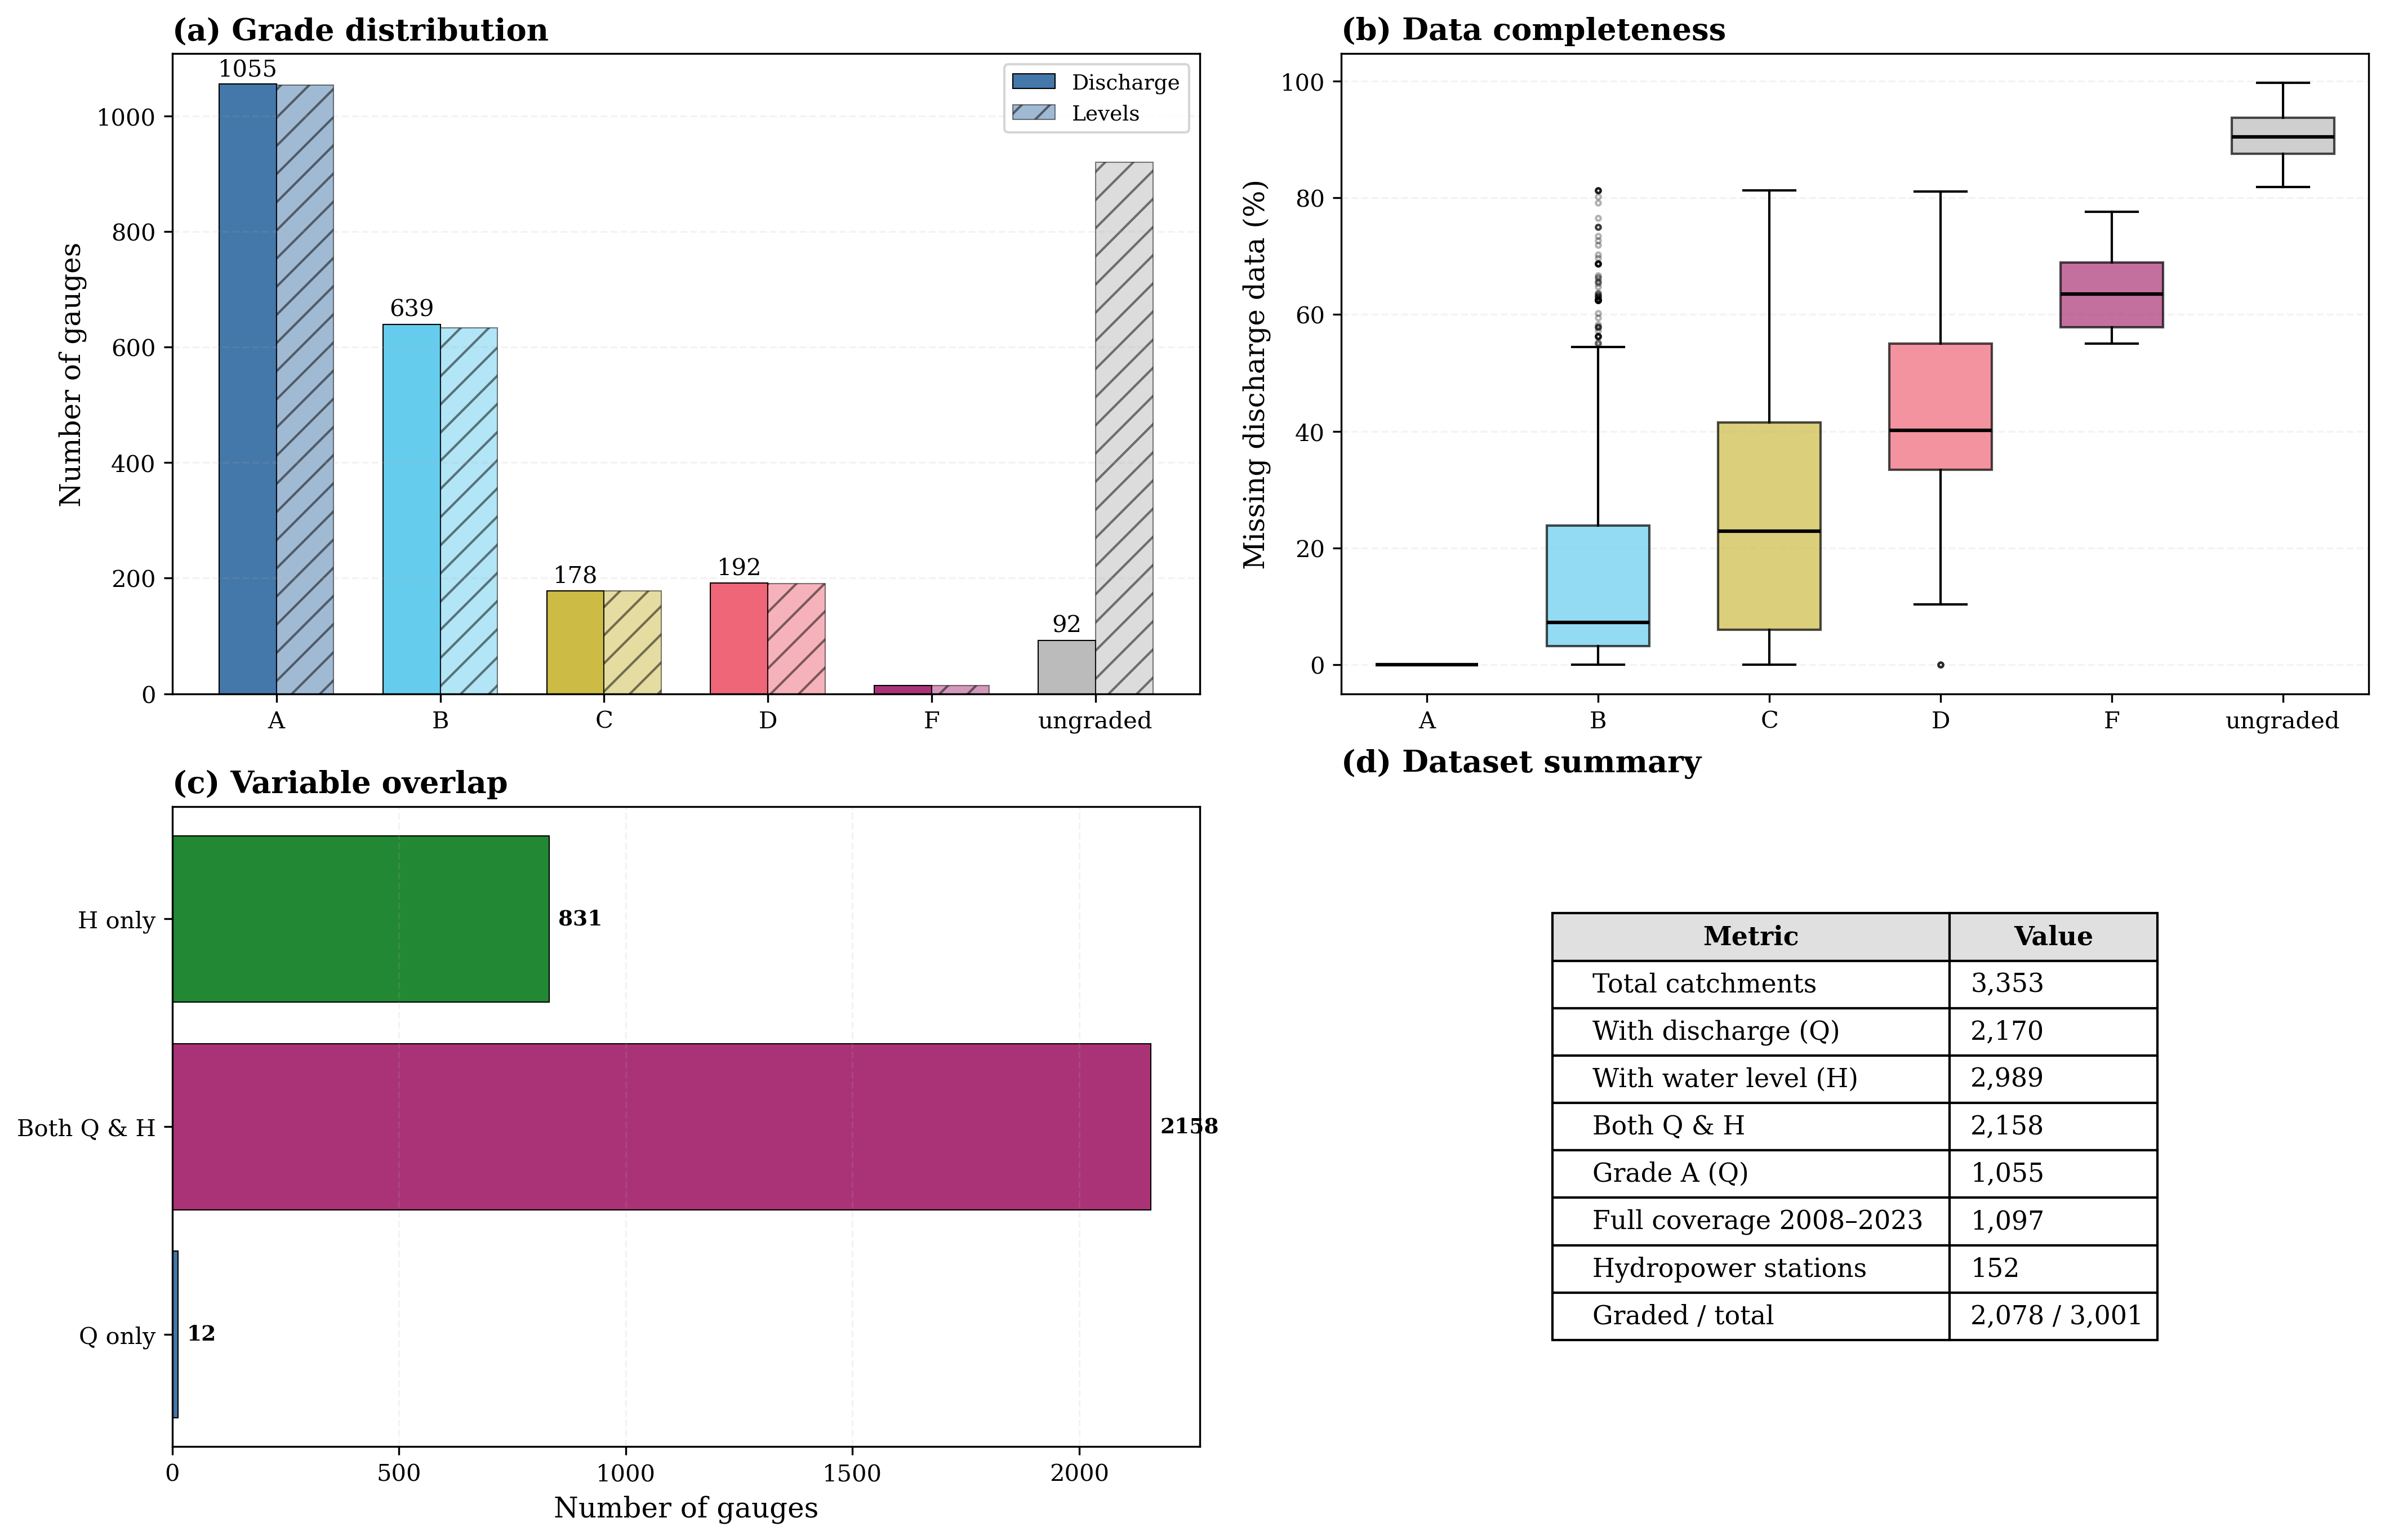
\includegraphics[width=0.95\columnwidth]{../images/fig_quality_assessment.png}
\caption{Quality assessment summary for the CAMELS-RU discharge network: data completeness, quality grade distribution, and temporal coverage across the \years study period.}
\label{fig:quality_assessment}
\end{figure}

\begin{figure}[htbp]
\centering
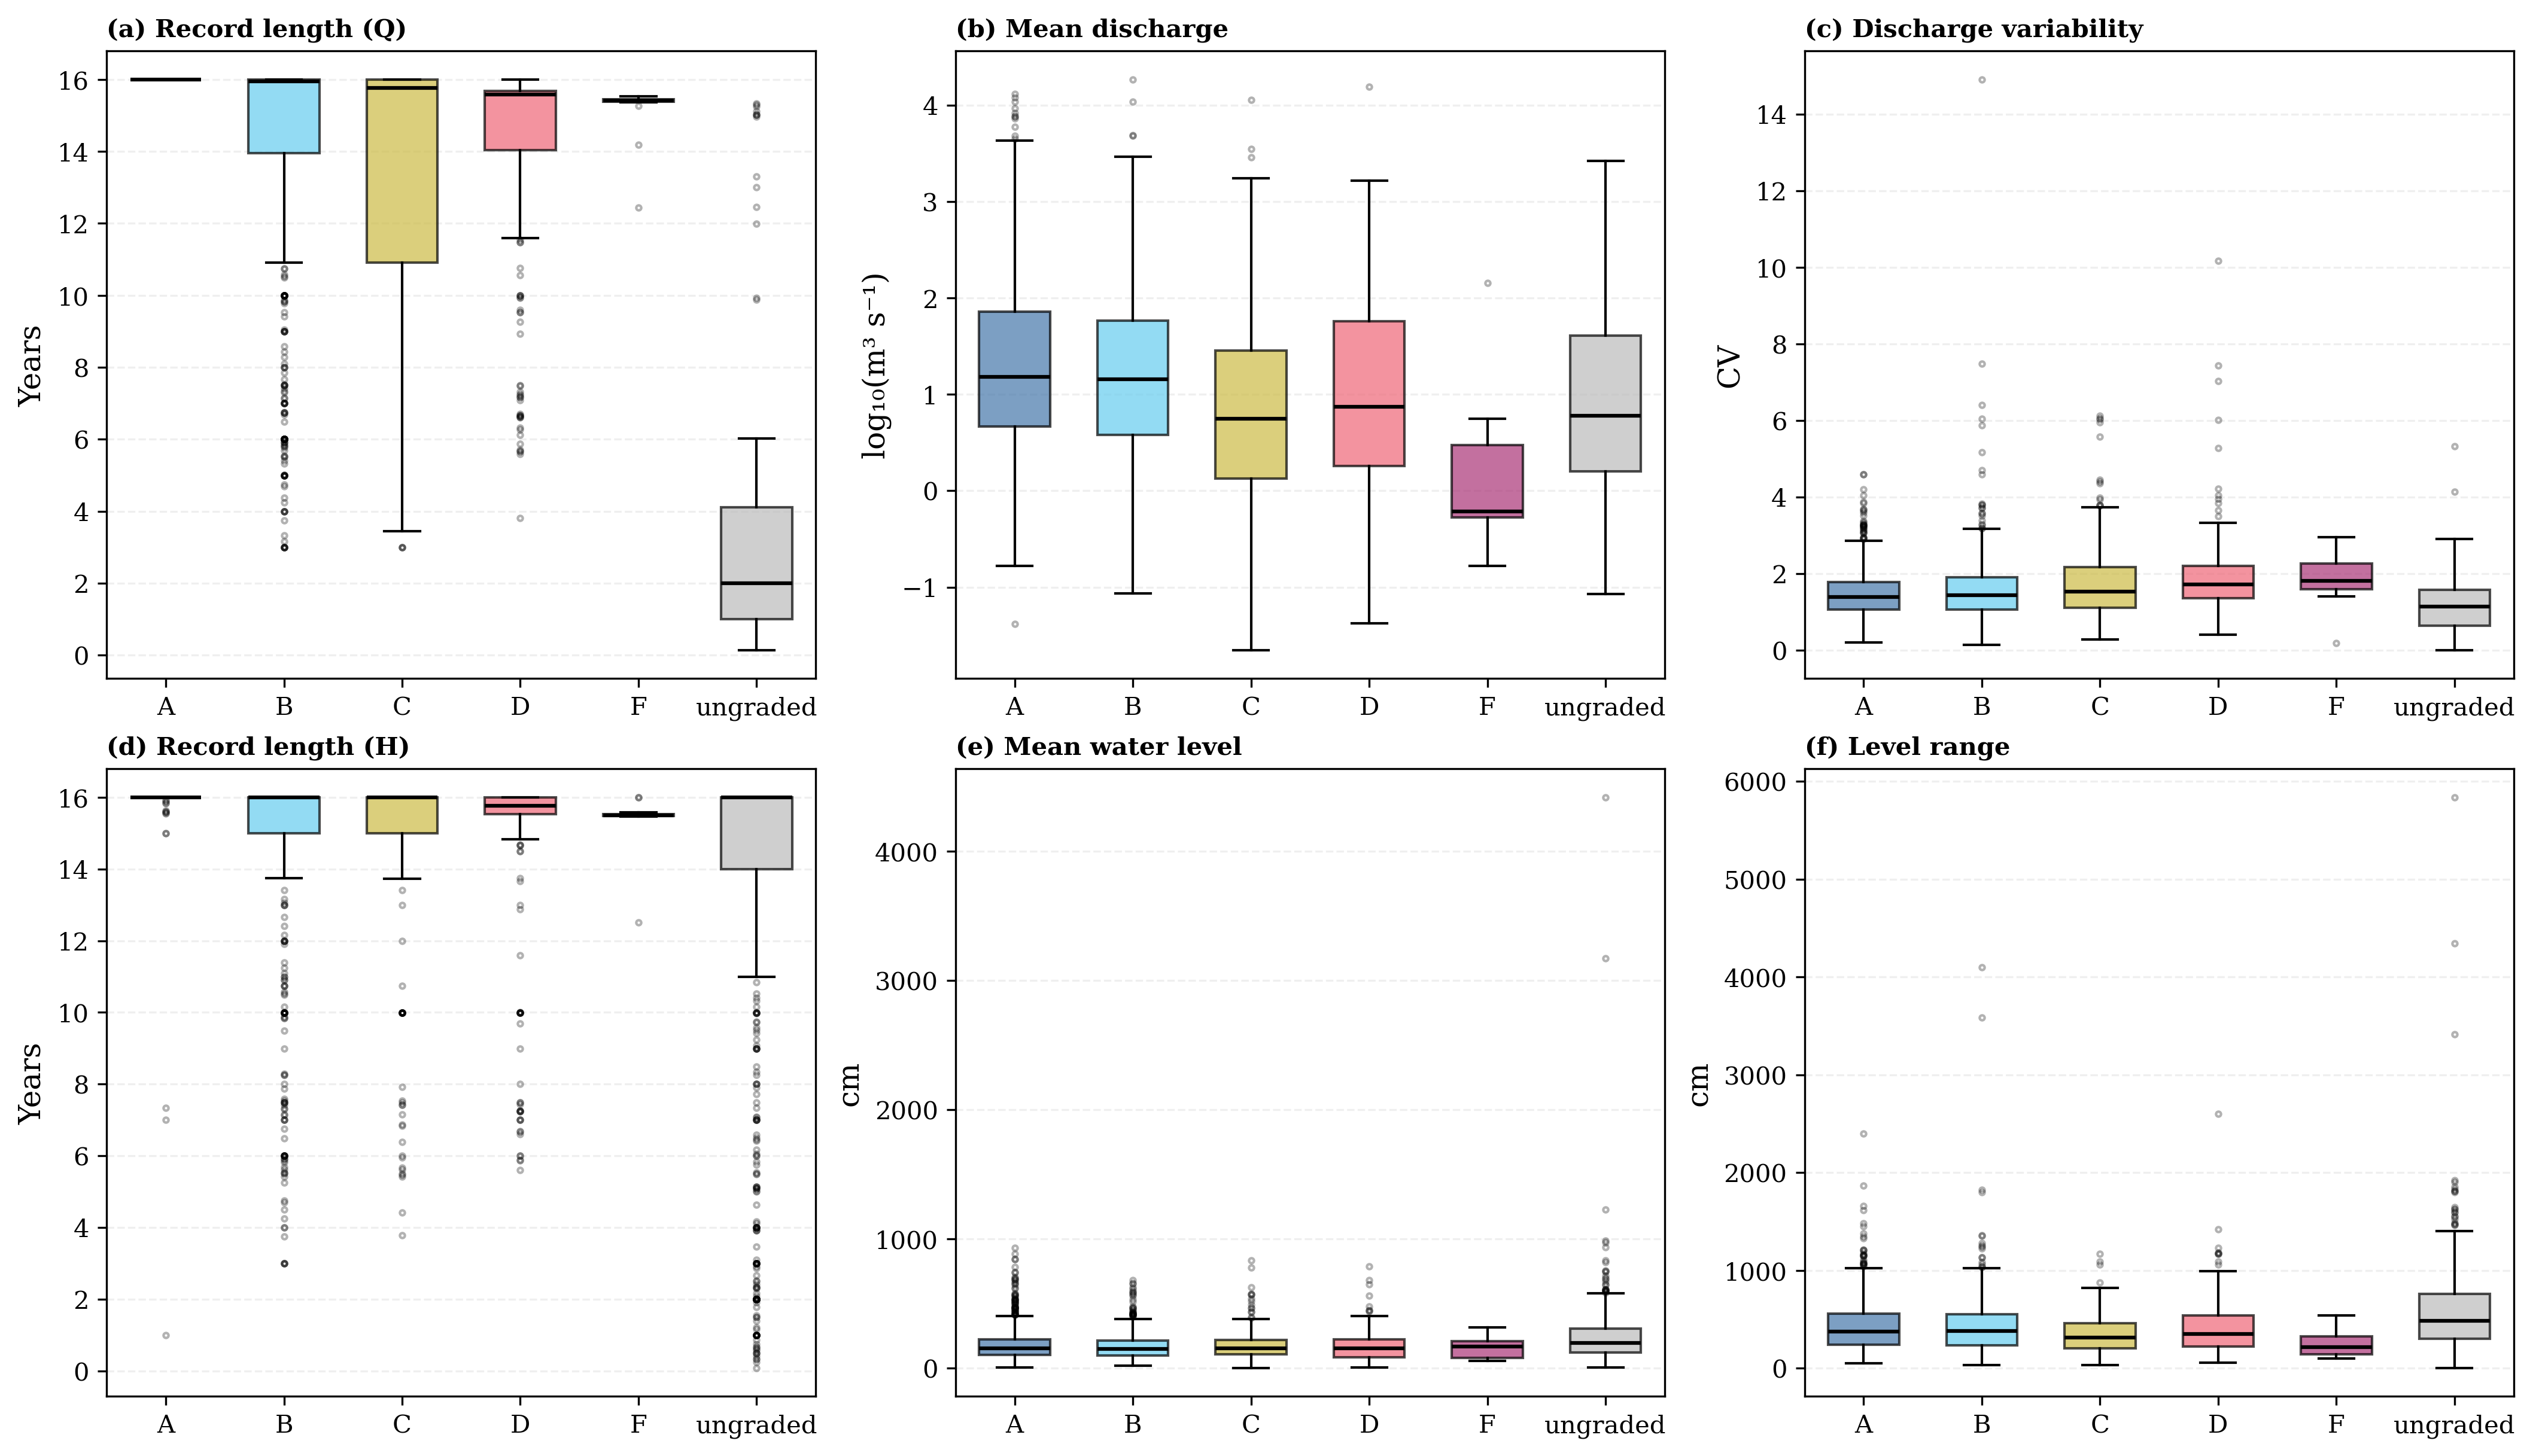
\includegraphics[width=0.95\columnwidth]{../images/fig_hydro_characteristics.png}
\caption{Discharge and water level characteristics across quality grades: summary statistics for the \ndischarge discharge gauges and \nwaterlevel water level gauges.}
\label{fig:hydro_characteristics}
\end{figure}

\subsection{Meteorological Forcing Data}
\subsubsection{ERA5-Land Reanalysis}
Meteorological forcing derived from ERA5-Land reanalysis~\citep{Munoz2021}, providing 0.1$^\circ$ ($\sim$9~km) hourly data aggregated to daily resolution.
Variables extracted:
\begin{itemize}
    \item Air temperature: mean, minimum, maximum ($^\circ$C)
    \item Potential evapotranspiration (mm/day, computed via Penman-Monteith)
    \item Precipitation (mm/day): mean annual \erafiveannual across catchments
\end{itemize}

For each catchment, basin-averaged forcing computed by weighting ERA5-Land grid cells by fractional catchment coverage, applying the standard environmental lapse rate ($-6.5^\circ$C/km) for elevation correction in mountain basins.

\subsubsection{MSWEP Precipitation}
Precipitation data sourced from Multi-Source Weighted-Ensemble Precipitation (MSWEP) version 2.8~\citep{Beck2019MSWEP}, a global precipitation dataset merging gauge observations, satellite estimates, and reanalysis data at 0.1$^\circ$ resolution.
Mean annual precipitation: \mswepannual across CAMELS-RU catchments.
MSWEP outperforms reanalysis-only products in gauge-sparse and snowfall-dominated regions~\citep{Beck2017MSWEP}.
Daily precipitation (mm/day) aggregated to catchment scale using area-weighted averaging of grid cells intersecting each watershed boundary.

\subsubsection{Inter-Dataset Validation}
Three precipitation products (ERA5-Land, MSWEP, GPCP) were cross-validated to assess forcing reliability.
Daily correlations range from $r = \eragpcpcorr$ (ERA5-Land vs.\ GPCP) to $r = \eramsweprcorr$ (ERA5-Land vs.\ MSWEP), with systematic differences in annual totals reflecting different data sources and spatial resolutions (see Sect.~\ref{sec:technical_validation}).

\subsection{Watershed Boundaries: Manual Verification}
\subsubsection{Base Delineation}
Initial catchment boundaries delineated using the MERIT Hydro digital elevation model (DEM;~\citealt{Yamazaki2019}) (3-arcsecond, $\sim$90~m resolution globally) and associated flow direction/accumulation grids.
MERIT Hydro reduces elevation errors in flat and forested terrain compared to earlier global DEMs by incorporating satellite altimetry and river network constraints.

Automated pour-point snapping algorithm identified nearest high-accumulation pixel (upstream area within 5\% of gauge catchment area reported by Roshydromet) within 500~m search radius of gauge coordinates.
Watershed delineation performed using standard D8 flow routing algorithm.

\subsubsection{Manual Expert Verification}
Every watershed boundary (\ntotal catchments) was manually verified and adjusted by a hydrographic expert using:
\begin{itemize}
    \item High-resolution satellite imagery (Google Earth, Sentinel-2 10~m)
    \item MERIT Hydro river network overlay
    \item Official Roshydromet topographic maps (1:100,000 scale)
    \item Local terrain knowledge and hydrographic principles
\end{itemize}

Manual adjustments corrected:
\begin{itemize}
    \item DEM artifacts in flat terrain (West Siberian Lowland, river deltas)
    \item Flow direction errors at confluences and braided reaches
    \item Canal diversions and reservoirs altering natural drainage
    \item Karst hydrology and subsurface flow contributions
\end{itemize}

\subsubsection{Validation Against Official Data}
Comparison with official Roshydromet catchment areas yielded:
\begin{itemize}
    \item Mean areal error: \meanerror (absolute difference)
    \item \withinfive of catchments within 5\% error
    \item \withinten of catchments within 10\% error
    \item Largest errors ($>$15\%) occur in complex karst terrain (Ural Mountains) and anthropogenically modified basins (irrigation canals, inter-basin transfers)
\end{itemize}

For comparison, \citet{Lehner2008} and \citet{Yamazaki2019} report 10--15\% mean areal errors from automated delineation in flat and permafrost terrain.

Known limitations of the dataset (temporal coverage, nested catchments, attribute temporal mismatch, and others) are consolidated in Sect.~\ref{sec:limitations}.

\subsection{Physiographic Attributes: HydroATLAS}
For each of the \ntotal manually verified catchment boundaries, all variables from the HydroATLAS v1.0 database~\citep{Linke2019} were extracted by spatially aggregating raster layers within watershed polygons using area-weighted averaging.
This produces 288 catchment-specific attribute values spanning hydrology, physiography, climate (including monthly temperature and precipitation), land cover, soil and geology, and anthropogenic variables.
The full attribute set is provided in the released CSV file.

Table~\ref{tab:hydroatlas_attributes} lists a recommended primary subset of \nattributes attributes selected by retaining upstream-aggregated annual variables and removing 12 features with pairwise $|r| > 0.7$ (e.g., slope correlated with elevation; aridity index redundant with precipitation and potential evapotranspiration, PET).
All removed attributes---including aridity index, slope, temperature, and soil properties---remain available in the full released attribute file for users who need them.

\begin{table*}[htbp]
\centering
\caption{Static catchment attributes derived from HydroATLAS v1.0 included in CAMELS-RU (\nattributes primary subset). Initial selection retained attributes matching upstream and sub-basin aggregation conventions; 12 inter-correlated features were subsequently removed (see Sect.~\ref{sec:data_sources_methods}). The full set of 288 HydroATLAS attributes is provided in the released CSV.}
\label{tab:hydroatlas_attributes}
\small
\begin{threeparttable}
\begin{tabular}{lllp{7cm}}
\toprule
\textbf{Category} & \textbf{Attribute} & \textbf{Unit} & \textbf{Description} \\
\midrule
\multirow{5}{*}{Climate \& water balance}
& ele\_mt\_uav & m & Mean elevation \\
& pre\_mm\_uyr & mm/yr & Mean annual precipitation \\
& pet\_mm\_uyr & mm/yr & Mean annual potential evapotranspiration \\
& aet\_mm\_uyr & mm/yr & Mean annual actual evapotranspiration \\
& snw\_pc\_uyr & \% & Mean annual snow cover extent \\
\midrule
\multirow{5}{*}{Land cover}
& for\_pc\_use & \% & Forest cover \\
& crp\_pc\_use & \% & Cropland cover \\
& pst\_pc\_use & \% & Pasture/grassland cover \\
& ire\_pc\_use & \% & Irrigated area \\
& pac\_pc\_use & \% & Protected area coverage \\
\midrule
\multirow{2}{*}{Cryosphere}
& gla\_pc\_use & \% & Glacier cover \\
& prm\_pc\_use & \% & Permafrost extent \\
\midrule
\multirow{3}{*}{Soil}
& cly\_pc\_uav & \% & Clay content (mean) \\
& slt\_pc\_uav & \% & Silt content (mean) \\
& snd\_pc\_uav & \% & Sand content (mean) \\
\midrule
\multirow{2}{*}{Hydrogeology}
& gwt\_cm\_sav & cm & Groundwater table depth \\
& kar\_pc\_use & \% & Karst area extent \\
\midrule
\multirow{2}{*}{Water bodies}
& inu\_pc\_ult & \% & Inundation extent \\
& lka\_pc\_use & \% & Lake/reservoir area \\
\midrule
\multirow{3}{*}{Human impact}
& ppd\_pk\_uav & pers/km$^2$ & Population density \\
& urb\_pc\_use & \% & Urban/built-up area \\
& gdp\_ud\_sav & USD/km$^2$ & GDP density \\
\bottomrule
\end{tabular}
\begin{tablenotes}
\small
\item All attributes are watershed-level aggregates computed individually for each manually verified catchment boundary using area-weighted spatial averaging.
\item Attribute codes follow HydroATLAS naming: suffix indicates aggregation (uav = upstream area-weighted average, use = upstream spatial extent, uyr = upstream annual mean, sav = sub-basin average, ult = upstream ultimate).
\end{tablenotes}
\end{threeparttable}
\end{table*}


\subsection{Hydrological Signatures}
We computed \nsignatures hydrological signatures (Table~\ref{tab:hydro_signatures}) characterizing discharge magnitude, variability, timing, and extremes for gauges meeting the per-year completeness criterion ($>$70\% for at least 5 hydrological years; $N = \nsigngauges$, or $N = \nhalfflowgauges$ for half-flow date which requires $>$82\%), following established methodologies~\citep{Sawicz2011,McMillan2017}.

Signatures were computed separately for individual hydrological years (October--September) and then averaged to produce catchment-characteristic values.
Key methodological choices:
\begin{itemize}
    \item Runoff ratio uses ERA5-Land precipitation as denominator; ratios differ with MSWEP ($\sim$0.36) or GPCP ($\sim$0.33) due to lower annual totals
    \item Flow duration curve (FDC) slope computed as $[\ln(Q_{33}) - \ln(Q_{66})] / (66 - 33) \times 100$ where $Q_p$ is discharge at the $p$-th exceedance percentile; positive values indicate steeper curves (note: sign convention opposite to \citealt{Sawicz2011})
    \item Baseflow index (BFI) computed using an ensemble of 1{,}000 Lyne--Hollick digital filter~\citep{Nathan1990} runs with $\alpha \sim U[0.9, 0.98]$ (3-pass), following \citet{Euser2013}
    \item Half-flow date requires $>$82\% annual completeness ($\geq$300 days) because partial years can shift the cumulative midpoint
    \item Richards--Baker flashiness index: $\sum|Q_i - Q_{i-1}| / \sum Q_i$, dimensionless measure of day-to-day flow variability
    \item High-flow and low-flow durations: mean consecutive days above $2\times$ median (high) or below $0.2\times$ mean (low) discharge
\end{itemize}

\begin{table}[htbp]
\centering
\caption{Hydrological signatures computed for CAMELS-RU catchments. All signatures derived from daily discharge time series for gauges with $>$70\% data completeness per hydrological year and at least 5 qualifying years ($n = \nsigngauges$; half-flow date requires $>$82\% completeness, $n = \nhalfflowgauges$). FDC slope is positive for steeper curves (opposite sign convention to \citealt{Sawicz2011}).}
\label{tab:hydro_signatures}
\begin{tabular}{llp{5.5cm}}
\toprule
\textbf{Signature} & \textbf{Unit} & \textbf{Description} \\
\midrule
\multicolumn{3}{l}{\textit{Magnitude}} \\
\quad q\_mean & mm/day & Mean daily discharge \\
\quad runoff\_ratio & -- & Annual $Q/P$ ratio (ERA5-Land precipitation) \\
\midrule
\multicolumn{3}{l}{\textit{Variability}} \\
\quad q\_cv & -- & Coefficient of variation of daily discharge \\
\quad FDC\_slope & -- & FDC slope between 33rd and 66th exceedance percentiles (log-space; positive = steeper) \\
\quad flashiness\_index & -- & Richards--Baker index: $\sum|Q_{i}-Q_{i-1}|/\sum Q_i$ \\
\midrule
\multicolumn{3}{l}{\textit{Extremes}} \\
\quad Q5 & mm/day & 5th exceedance percentile (high flows) \\
\quad Q95 & mm/day & 95th exceedance percentile (low flows) \\
\quad high\_flow\_freq & \% of days & Days exceeding $2\times$ median discharge \\
\quad high\_flow\_dur & days & Mean duration of high-flow events ($>2\times$ median) \\
\midrule
\multicolumn{3}{l}{\textit{Baseflow}} \\
\quad baseflow\_index & -- & Baseflow fraction; ensemble of 1{,}000 Lyne--Hollick filter runs, $\alpha \sim U[0.9, 0.98]$, 3-pass \\
\midrule
\multicolumn{3}{l}{\textit{Low Flow}} \\
\quad low\_flow\_freq & \% of days & Days below $0.2\times$ mean discharge \\
\quad low\_flow\_dur & days & Mean duration of low-flow events ($<0.2\times$ mean) \\
\midrule
\multicolumn{3}{l}{\textit{Seasonality}} \\
\quad half\_flow\_date & day of hydro yr & Day of hydrological year (Oct~1 = day~1) when 50\% of annual streamflow volume has passed \\
\bottomrule
\end{tabular}
\end{table}



